\documentclass{cmc}

\begin{document}

\pagestyle{fancy}
\lhead{\textit{\textbf{Computational Motor Control, Spring 2019} \\
    Python exercise, Lab 5, GRADED}} \rhead{ROVINA Hannes, INDUMI Mirko,\\ NIEDERHAUSER Loïc}

\section*{Student names: \\NIEDERHAUSER Loïc, ROVINA Hannes, INDUMI Mirko}
\textit{Instructions: Update this file (or recreate a similar one,
  e.g.\ in Word) to prepare your answers to the questions. Feel free
  to add text, equations and figures as needed. Hand-written notes,
  e.g.\ for the development of equations, can also be included e.g.\
  as pictures (from your cell phone or from a scanner).
  \textbf{\corr{This lab is graded.}} and must be submitted before
  the \textbf{\corr{Deadline : 11-04-2018 Midnight}}.  \\ Please
  submit both the source file (*.doc/*.tex) and a pdf of your
  document, as well as all the used and updated Python functions in a
  single zipped file called \corr{lab5\_name1\_name2\_name3.zip} where
  name\# are the team member’s last names.  \corr{Please submit only
    one report per team!}}
\\

\textit{The file \fileref{lab\#.py} is provided to run all exercises
  in Python.
  % Each \fileref{exercise\#.py} can be run to run an exercise
  % individually.
  % The list of exercises and their dependencies are shown in
  % Figure~\ref{fig:files}.
  When a file is run, message logs will be printed to indicate
  information such as what is currently being run and and what is left
  to be implemented. All warning messages are only present to guide
  you in the implementation, and can be deleted whenever the
  corresponding code has been implemented correctly.}


% \textit{In this exercise, you will explore the different modeling
%   techniques that can be used to control a single joint and
%   segment. We initially start by exploring a single joint controlled
%   by a pair of antagonist spring like muscles and then extend the
%   model by adding dampers to it. These only represent the passive
%   dynamics observed in a real musculoskeletal system. To make the
%   behavior more realistic we then study more complex hill muscle model
%   in detail. }

%%%%%%%%%% TO BE ADDED [WIP] %%%%%%%%%%

\begin{figure}[ht]
  \centering 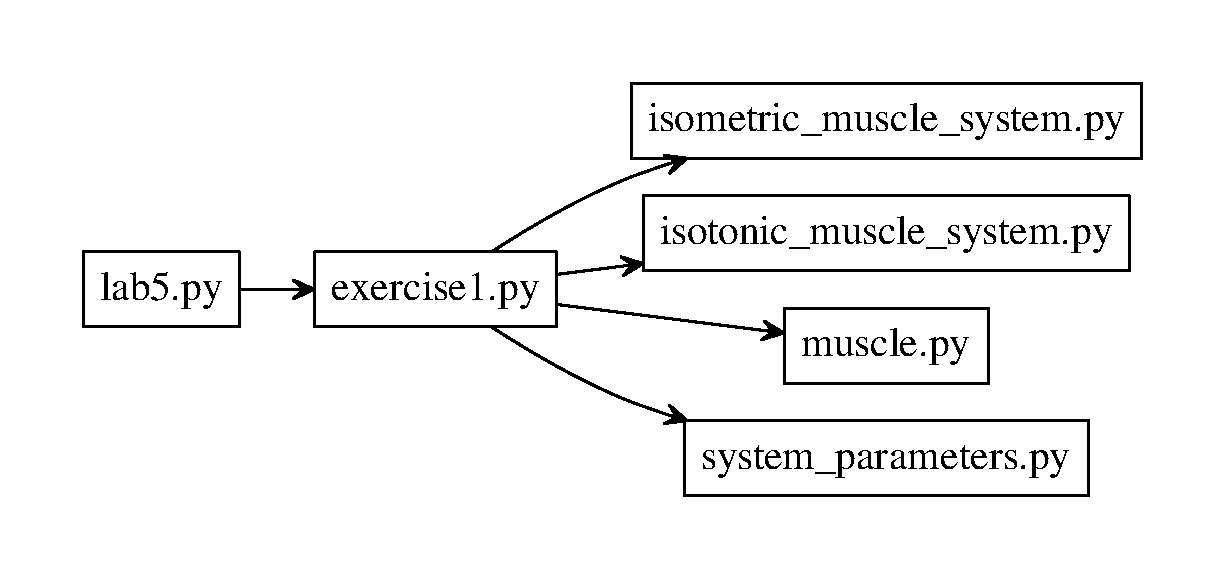
\includegraphics[width=0.5\textwidth]{figures/files}
  \caption{\label{fig:files} Exercise files dependencies. In this
  lab, you will be modifying \fileref{exercise1.py}.}
\end{figure}

\subsection*{Files to complete the exercises}
\label{sec:intro}

\begin{itemize}
\item \fileref{lab5.py} : Main file
\item \fileref{exercise1.py} : Main file to complete exercise 1
\item \fileref{system\_parameters.py} : Parameter class for Pendulum,
  Muscles and Neural Network (Create an instance and change properties
  using the instance. You do not have to modify the file)
\item \fileref{isometric\_muscle\_system.py} : Class to setup your
  isometric muscle test experiments
\item \fileref{isotonic\_muscle\_system.py} : Class to setup your
  isotonic muscle test experiments
\item \fileref{muscle.py} : Muscle class (You do not have to modify
  the file)
\end{itemize}

\textbf{NOTE : } '\textit{You do not have to modify}' does not mean
you should not, it means it is not necessary to complete the
exercises. But, \corr{you are expected to look into each of these
  files and understand how everything works}. You are free to explore
and change any file if you feel so.
\clearpage

\section*{Exercise 1 : Hill muscle model}
\label{sec:question-2}

Previous week you explored the role of different passive components
and the effects of its parameters on the system. In this exercise, we
try to understand the contractile or the active element of the hill
muscle model. The components of the hill muscle are described in
figure \ref{fig:hill_muscle}. The equations used to model the hill
muscle can be found in the pdf \fileref{HillMuscleEquations.pdf}

\begin{figure}[H]
  \centering 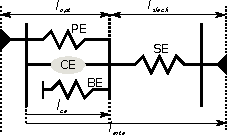
\includegraphics[scale=2.5]{figures/hill_muscle}
  \caption{Hill muscle model}
  \label{fig:hill_muscle}
\end{figure}

Where,

\begin{itemize}
\item $PE$ : Parallel element (Prevents muscle from over stretching)
\item $BE$ : Muscle Belly (Prevents muscle from collapsing on itself)
\item $SE$ : Series element or the muscle tendon element
\item $CE$ : Contractile Element or the active element
\item $l_{opt}$ : Muscle optimal fiber length
\item $l_{slack}$ : Muscle tendon slack length
\item $l_{CE}$ : Contractile element length
\item $l_{MTC}$ : Muscle Tendon Complex length
\end{itemize}


\begin{figure}[H]
  \centering
  \begin{subfigure}[b]{0.49\textwidth}
    { \centering
      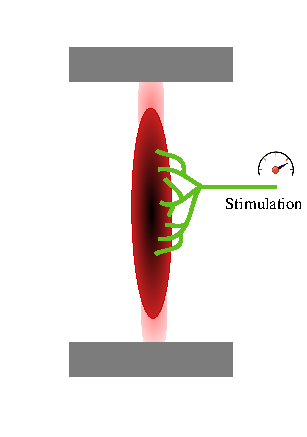
\includegraphics[width=\textwidth]{figures/isometric_muscle} }
    \caption{Isometric muscle setup :\\ To study the relationship
      between Force-Length.}
    \label{fig:isometric_muscle}
  \end{subfigure}
  \begin{subfigure}[b]{0.49\textwidth}
    { \centering
      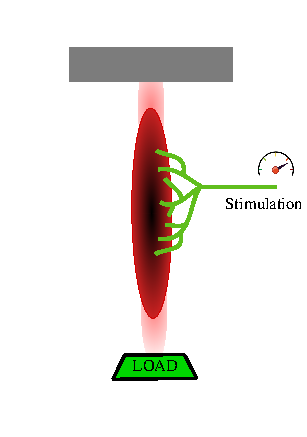
\includegraphics[width=\textwidth]{figures/isotonic_muscle} }
    \caption{Isotonic muscle setup :\\ To study the relationship
      between Force-Velocity.}
    \label{fig:isotonic_muscle}
  \end{subfigure}
  \caption{Muscle Length-Velocity-Force Setup}
  \label{fig:muscle-setup}
\end{figure}

\subsection*{Muscle Force-Length Relationship}
\label{sec:muscle-force-length}
In this exercise you will explore the relation between the length and
velocity of the muscle. In order to do this we replicate the set-up
show in figure \ref{fig:muscle-setup}.Here the length of the muscle is
held constant by attaching it's tendon to two fixed points. While
applying a constant stimulation, observing the force produced will
give the relationship between muscle contractile element length and
force.
\subsection*{1.a For a given stimulation, explore the relationship
  between active and passive muscle forces and the length of the
  contractile element.  Plot the force-length relationship curve.
  Discuss the different regions in the plot. Use the
  \fileref{isometric\_muscle\_system.py::IsometricMuscleSystem} instance
  to setup your experiment in \fileref{exercise1.py}}


\begin{figure}[H]
    \centering
    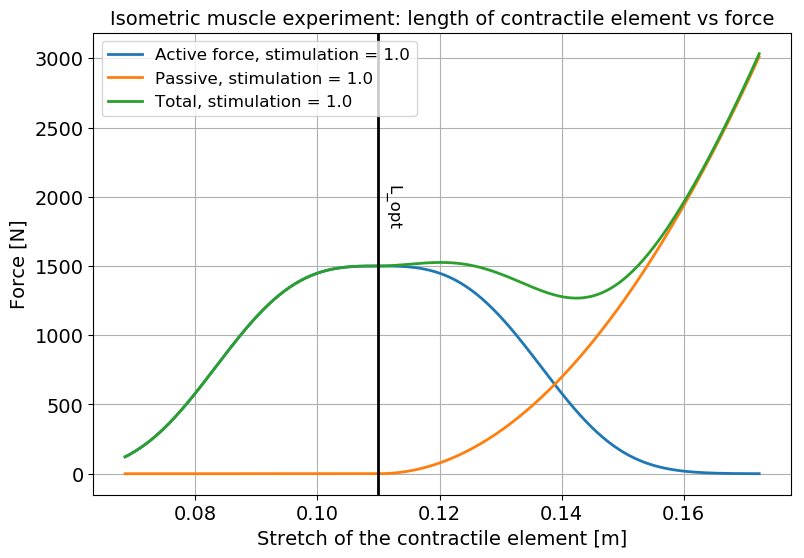
\includegraphics[width=0.6\textwidth]{figures/1_a_lce_vs_str.png}
    \caption[Isometric experiment]{Force length relationship for an isometric muscle experiment with a total muscle stretch from 0.2[m] (where $l_{ce}\approx0.6\cdot l_{opt}$)\footnotemark  to 0.31[m] (where $l_{ce}\approx1.5\cdot l_{opt}$) and stimulation of 1.}
    \label{fig:Exercise1a}
\end{figure}

  \footnotetext{It is the maximal compression that can be applied to this model. Beyond this point the forces drops to zero and nothing happens. This is one of the limitations of our current model.} % Footnote from the caption. Has to be done this way.

From the muscle model setting we know that the length of the contractile element where the muscle has the maximal strength ($l_{opt}$ in figure \ref{fig:hill_muscle}) is 0.11 [m]. Therefore we can deduce from the plot of figure \ref{fig:Exercise1a} that the active force decreases by either contracting or extension. This result is supported with the following biological explanation:
\begin{figure}[H]

\centering
\begin{subfigure}[b]{0.49\textwidth}
         \centering
         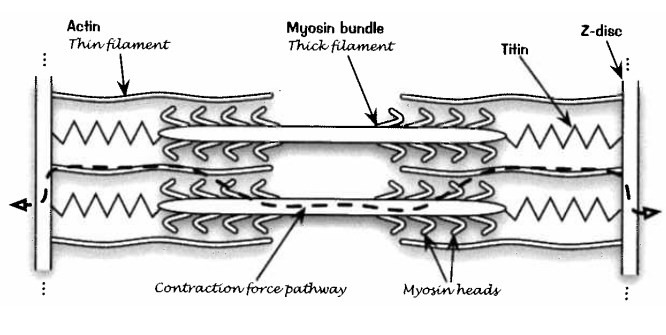
\includegraphics[width=\textwidth]{figures/Sacromere.jpg}
         \caption{Detail of a sarcomere}
         \label{fig:sarcomere}
     \end{subfigure}
\begin{subfigure}[b]{0.49\textwidth}
         \centering
         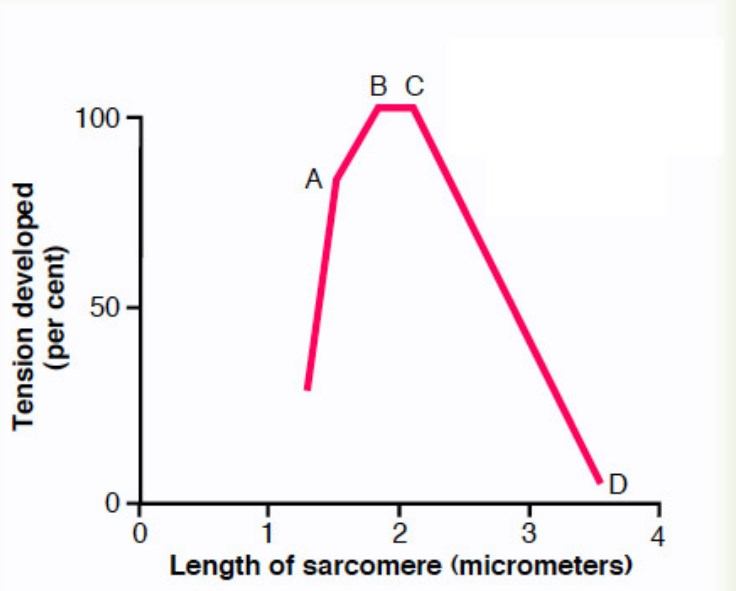
\includegraphics[width=\textwidth]{figures/ActiveForce.jpg}
         \caption{Active force generrated by a sarcomere}
         \label{fig:activeforce}
     \end{subfigure}
    
     \caption{Source: Slides from course. "Biomechanics of the musculo-sceletal system" by Prof. D. Pioletti, Fall 2018}
     \label{fig:Exercise1c}
\end{figure}
\paragraph{Biological explanation:} A muscle fiber consists of an addition of sarcomeres when reduced to its basic unit. Each of these sarcomeres consist of a myosin bundle with its heads, that can move on the actin filament (see figure \ref{fig:sarcomere}). As the head "walk" on the actin filaments the Z-discs move together and on macroscale the muscle is contracting. The more myosin are attached on the actin bundle, the more force the sarcomere can produce. 

By analyzing the sarcomere in figure \ref{fig:sarcomere} the active force in figure \ref{fig:activeforce} can be understood. At point D, the Myosin bundle is almost completely torn out of the actin filament, therefore only few heads are attached to it and little force is produced. By contracting the muscle, the sarcomere contract and we arrive at point C which represents the state shown on figure \ref{fig:sarcomere}, all heads are just on the actin filament. By contracting even more, point B is reached. There the actin filaments are moved so close together that they touch. It is interesting to notice that without external constraints, the muscle will rest at a length around B and C. By even further contracting the muscle, the actin filament start to overlap producing more resistance and the resulting force produced by the sarcomere decreases rapidly (point A). Ultimately the myosin bundles will be blocked by the Z-discs resulting in the impossibility of producing any force.

\paragraph{Plot analysis:} Finally on plot \ref{fig:Exercise1a} the total force is nonlinear and can be explained by the superposition of two curves: the passive and the active forces. In this model the active force is generated by a sarcomere-like element and attempts to mimic the biological response described above. The passive force is generated by a non linear elastic part in our model and mimics the elasticity of the muscles and tendons. For small extensions the active force will constitute a more important part of the total force. However, when the muscle is streched further, the active force will decrease due to the loss of force in the muscle and the elastic or passive force will increase more due to its nature, thus constituting the major component of the total force.
\vfill
\clearpage

\subsection*{1.b In (1.a), you explored the muscle force-length
  relationship for a given stimulation. What happens to the
  relationship when the stimulation is varied between [0 - 1]? Support
  your response with one plot showing the different force-length
  relationship curves.}

The first thing that we can expect is that the material property of the muscle does not change with the simulation, therefore the passive force curve should stay the same if the stimulation is varied. This statement is in fact supported by the results\footnote{The legends for each passive force curve are not displayed for space related reasons. However, every passive force curve is plotted but doesn't show since they lie all under the purple curve.} obtained in figure \ref{fig:Exercise1b}.
\begin{figure}[H]
    \centering
    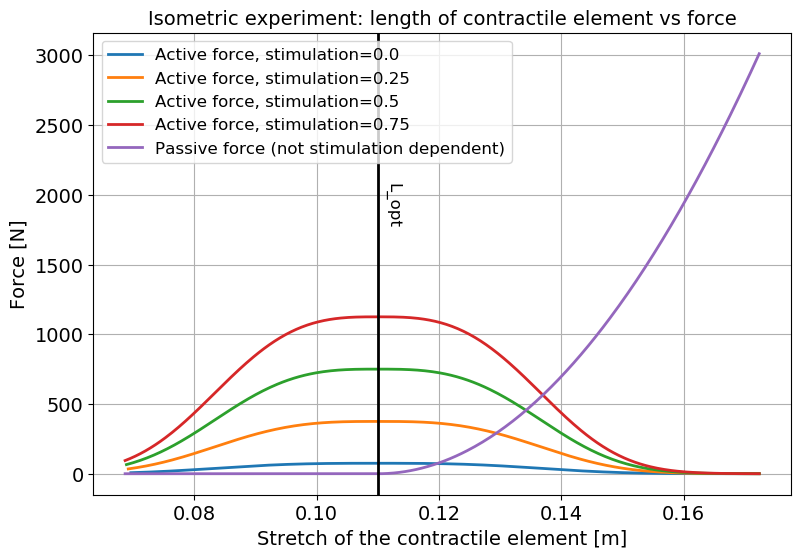
\includegraphics[width=0.6\textwidth]{figures/1_b_lce_stimulation.png}
    \caption[Isometric experiment with multiple intensities]{Force length relationship for multiple isometric muscle experiments with a total muscle stretch from 0.2[m] (where $l_{ce}\approx0.6\cdot l_{opt}$)\footnotemark  to 0.31[m] (where $l_{ce}\approx1.5\cdot l_{opt}$) and stimulation intensities from 0 to 1.}
    \label{fig:Exercise1b}
\end{figure}
\footnotetext{For the same reasons as in figure \ref{fig:Exercise1a}} % Still the only way to make a footnote inside a caption

Furthermore, we see that on one hand the active force of the muscle increases by increasing the stimulation which was expected since a more intense simulation should lead to a higher force. On the other hand the form of the force curve remains the same which was also expected since the biological behaviour of the muscle should remain the same. Finally one artifact needs to be addressed. It seems the when the muscle is left at rest (stimulation=0) the active force isn't null at all time. This is unexpected and does not match the biological model. This is due to the python implementation in which, to avoid dividing by zero, the minimal stimulation is set to 0.05, hence it is not possible to simulate a muscle at rest.
\vfill
\clearpage

\subsection*{1.c Describe how the fiber length ($l_{opt}$) influences
  the force-length curve.  (Compare a muscle comprised of short muscle
  fibers to a muscle comprised on long muscle fibers.). To change the
  parameter you can use
  \fileref{system\_parameters.py::MuscleParameters} before
  instantiating the muscle. No more than two plots are required. }

\begin{figure}[H]
\centering
    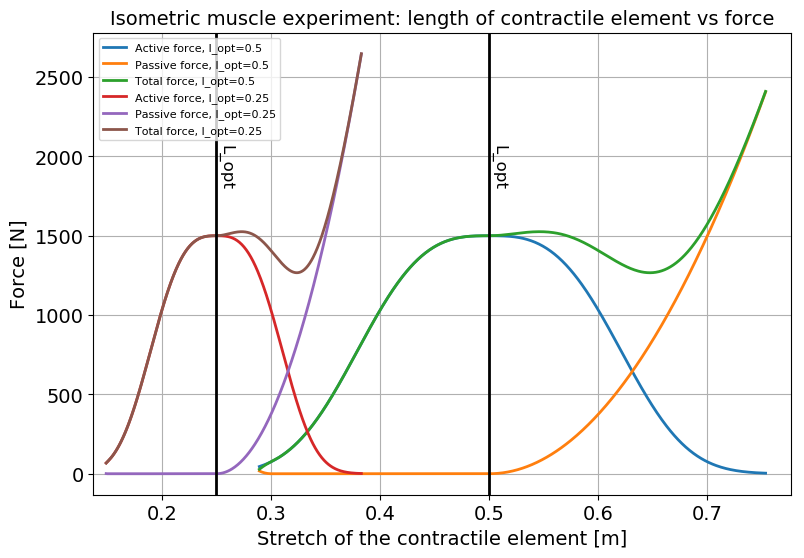
\includegraphics[width=0.8\textwidth]{figures/1_c_lce_iso_merged.png}
    \caption{Force length relationship for an isometric muscle ($l_{opt}$=0.25 [m] and 0.5 [m]) with a stimulation of 1}
    \label{fig:Exercise1c}
\end{figure}

From figure \ref{fig:Exercise1c} we can deduce that the amplitude of the active force produced is identical if the simulation remains the same. What changes is the length the muscle is contracted to since the muscle fiber have not the same length. Furthermore the stretch at which this force is produced changes which is expected since the length of the contractile element was explicitly changed. A shorter element should produce maximal strength at a shorter stretch as shown in figure \ref{fig:Exercise1c}. An other interesting point is that the passive stretch is higher for the shorter contractile element. Indeed the element being shorter, the tendon is more elongated for the same stretch, thus producing a higher force. 

\vfill
\clearpage

\subsection*{Muscle Velocity-Tension Relationship}
In this exercise you will explore the relation between the force and
velocity of the muscle. In order to do this we replicate the set-up
show in figure \ref{fig:muscle-setup}. Here the length of the muscle
is allowed to vary by attaching one of its end to a fixed point and
the other to a variable external load. While applying a constant load
initially and holding the muscle at constant length, a quick release
is performed to let the muscle contract and pull the weight. The
maximum velocity during this quick release will give us the
relationship between muscle contractile velocity and the force.


\corr{Note} : Since the velocity changes sign and you need to compute the maximum
velocity accordingly by checking if the muscle was stretched or compressed
at the end of the experiment.

\begin{equation}
  \label{eq:2}
 V_{ce} = \left\{
\begin{array}{ll}
      max(v_{ce}(t)) & l_{mtc} < (l_{opt} + l_{slack}) \\
      min(v_{ce}(t)) & else \\
\end{array}
\right.
\end{equation}

\subsection*{1.d For a stimulation of 1.0 and starting at optimal
  muscle length, explore the relationship between contractile element
  velocity and external load. Plot the Velocity-Tension relationship
  curve. Include shortening and lengthening regions. Use the
  \fileref{isotonic\_muscle\_system.py::IsotonicMuscleSystem} instance
  to setup your experiment in \fileref{exercise1.py}}

\begin{figure}[H]
    \centering
    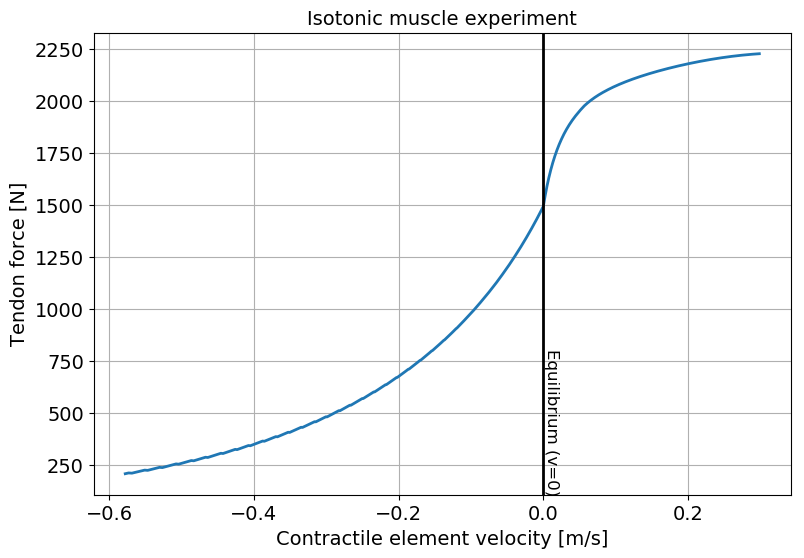
\includegraphics[width=0.6\textwidth]{figures/1_d_isotonic_load_var.png}
    \caption{Velocity force relationship for an isotonic muscle experiment with a load from 20[kg] to 300[kg] and a stimulation of 1}
    \label{fig:Exercise1d}
\end{figure}

Before analyzing figure \ref{fig:Exercise1d} one should know that a negative velocity means that the muscle is contracting, hence on figure \ref{fig:isotonic_muscle} the load is moving upwards. We see that for low loads at constant stimulation of the muscle, the muscle is able to create a force and lift the load. As the load increases, the muscle force increases until a breaking point is reached and the load can not be lifted anymore. The stimulation should be increased if higher loads are desired to be lifted.

It can be further stated that at the point with zero velocity, the experiment is at isometric condition and a force of 1500 Newtons is produced. The same result was obtained in exercise 1a for active and passive force added together at $l_{opt}$.

\subsection*{1.e For the muscle force-velocity relationship, why is
  the lengthening force greater than the force output during
  shortening? No plots necessary}

The force in the tendons is increasing with greater load because as soon the load is not supported anymore (lengthening), the passive force will get dominant and as we saw on the plot on figure \ref{fig:Exercise1a}, the passive force is able to reach higher intensities than the active force.


\subsection*{1.f What happens to the force-velocity relationship
  when the stimulation is varied between [0 - 1]? Support your
  response with one plot showing the different force-velocity
  relationship curves.  }

\begin{figure}[H]
\centering
\begin{subfigure}[b]{0.49\textwidth}
         \centering
         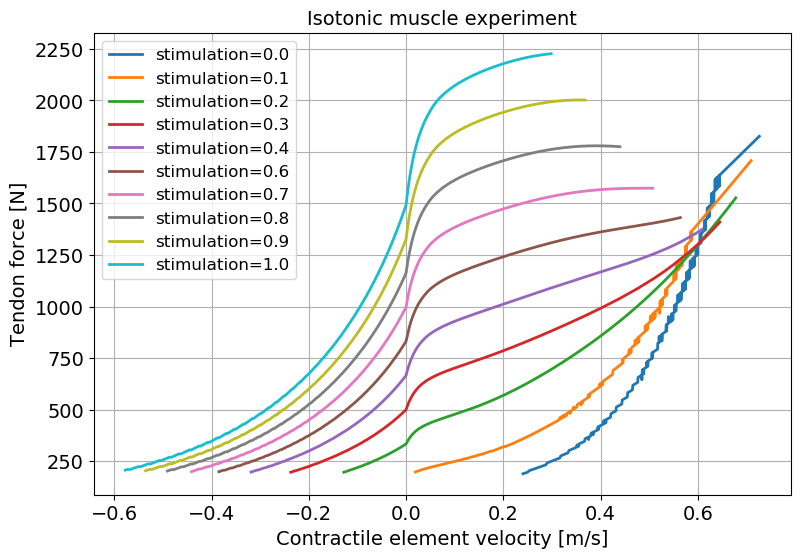
\includegraphics[width=\textwidth]{figures/1_d_isotonic_stim_var.png}
         \label{fig:isotonic_stim}
     \end{subfigure}
\begin{subfigure}[b]{0.49\textwidth}
         \centering
         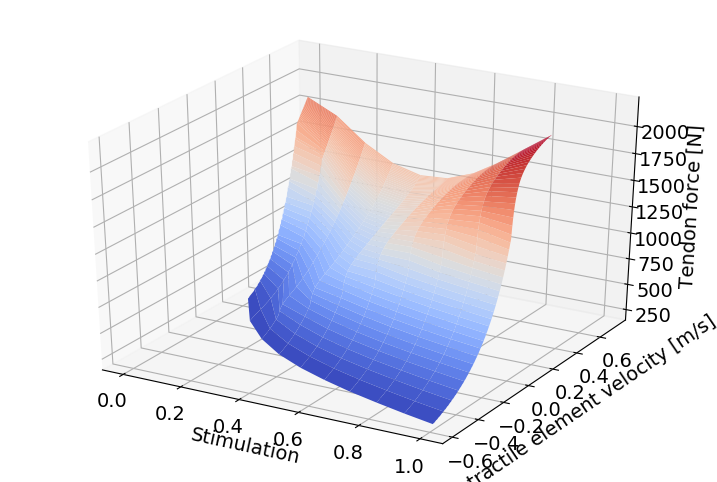
\includegraphics[width=\textwidth]{figures/1_d_isotonic_3d.png}
         \label{fig:isotonic_3d}
     \end{subfigure}
    
     \caption{Velocity force relationship for an isotonic muscle experiment with a load from 20[kg] to 300[kg] and a stimulation from 0 to 1.}
     \label{fig:Exercise1e}
\end{figure}

As already mentioned before the more the stimulus is increased the more weight can be supported. If the muscle is not stimulated at all, the load will obviously not be lifted at all. However as mentioned before a null stimulation is not allowed by the python implementation hence the zero stimulation curve should still be able to support a low weight ($\ll20[kg]$)
\end{document}

%%% Local Variables:
%%% mode: latex
%%% TeX-master: t
%%% End: